
\section{Comunicação} % (fold)
\label{sub:comunicação}
	De acordo com o apresentado nesta documentação de projeto, a solução proposta envolve diversos módulos funcionais, como o robô em si, a base fixa, e o sistema de controle. A partir de uma visão de alto nível do projeto, como a apresentada na Figura \ref{img:arq_comu}, é possível observar de maneira clara os módulos que deverão se comunicar para garantir o funcionamento do sistema como um todo.

	\begin{figure}[H]
		\centering
		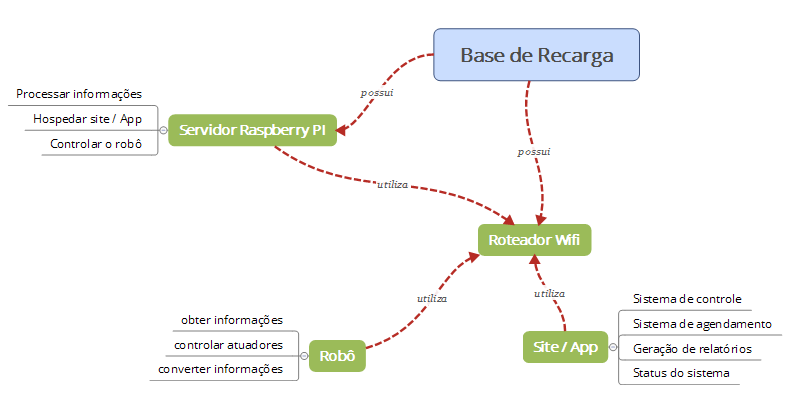
\includegraphics[scale=0.8]{figuras/arquitetura_comunicacao.png}
		\caption{Arquitetura de comunicação do sistema}
		\label{img:arq_comu}
	\end{figure}

	Com o objetivo de garantir que a solução seja confiável e resistente a situações críticas, como a falta de internet, por exemplo, o sistema foi planejado para disponibilizar uma sub-rede interna, tendo como fonte a base de recarga do robô. Cada módulo que necessita de comunicação deverá se conectar a rede, viabilizando o funcionamento do sistema mesmo em momentos com falha de internet, já que todos os envolvidos compartilham o mesmo ambiente.

	A comunicação entre o robô (\textit{arduino}) e a base (raspberry) fará uso desta rede wifi, a partir da utilização de um módulo wifi, o \textit{arduino} poderá acessar a rede, possibilitando a comunicação via tcp/ip. Já a \textit{raspberry} se conectará a rede via cabo \textit{ethernet}.

	O roteador utilizado é da familia D-link, seguindo o protocolo de certificação WPA2, que utiliza o EAS (Advanced Encryption Standard), como sistema de encriptação. Segundo \cite{wpa2}, este protocolo possui uma confiabilidade bem maior que a encontrada em seu antecessor, WPA. Ainda de acordo com \cite{wpa2}, este sistema de segurança envolve um algoritmo de criptografia robusto, utilizando chaves de 128 a 256 bits maximizando a segurança da rede.

	O núcleo da rede, ou seja, o ponto central da comunicação do sistema se encontra na base de recarga do robô, que está detalhada no tópico a seguir.

	\subsection{Base de recarga}

	A base de recarga do robô sustentará todo o sistema de inteligência da solução, assim como a sub-rede que possibilitará a comunicação entre os módulos. Será utilizada uma \textit{raspberry PI} como servidor central do sistema, processando e controlando toda a solução. O servidor será implementado utilizando a tecnologia Ruby on Rails, no sistema operacional \textit{Raspbian} (Debian).

	Além da sustentação da \textit{raspberry}, é necessário sustentar um roteador D-link 524 para implementação e sustentação da rede wifi que será utilizada como meio de comunicação do sistema, e 3 (três) emissores infra-vermelho, utilizados para retorno do robô à base.
	
% section comunicação (end)